\documentclass[11pt,a4paper]{article}
\usepackage[utf8x]{inputenc}
\usepackage{ucs}
\usepackage[spanish]{babel}
\usepackage[left=2cm,top=2cm,right=2cm,bottom=3cm]{geometry} 
\usepackage{amsmath}
\usepackage{amsfonts}
\usepackage{amssymb}
\usepackage{dcolumn}
\usepackage{float}
\usepackage{graphicx}
\usepackage{ esint }
\usepackage{fancyhdr}
\usepackage{enumerate} 
\pagestyle{fancy}
\usepackage{tocbibind}
\usepackage{setspace}
\usepackage{parskip}
\usepackage[hidelinks]{hyperref}
\usepackage{listings} 
\usepackage[svgnames]{xcolor}

\definecolor{codegreen}{rgb}{0,0.6,0}
\definecolor{codegray}{rgb}{0.5,0.5,0.5}
\definecolor{codepurple}{rgb}{0.58,0,0.82}
\definecolor{backcolour}{rgb}{0.95,0.95,0.92}


\definecolor{dkgreen}{rgb}{0,0.6,0}
\definecolor{gray}{rgb}{0.5,0.5,0.5}
\definecolor{mauve}{rgb}{0.58,0,0.82}


\lstset{basicstyle=\ttfamily}
\lstdefinestyle{mystyle}{
	%backgroundcolor=\color{backcolour},   
	commentstyle=\color{codegreen},
	keywordstyle=\color{magenta},
	numberstyle=\tiny\color{codegray},
	stringstyle=\color{codepurple},
	breakatwhitespace=false,         
	breaklines=true,                 
	keepspaces=true,                 
	numbers=left,                    
	%numbersep=5pt                  
}

\lstdefinestyle{customasm}{
  belowcaptionskip=1\baselineskip,
  frame=L,
  xleftmargin=\parindent,
  language= Python,
  basicstyle=\footnotesize\ttfamily,
  commentstyle=\itshape\color{purple!40!black},
}

\lstset{literate=
  {á}{{\'a}}1 {é}{{\'e}}1 {í}{{\'i}}1 {ó}{{\'o}}1 {ú}{{\'u}}1
  {Á}{{\'A}}1 {É}{{\'E}}1 {Í}{{\'I}}1 {Ó}{{\'O}}1 {Ú}{{\'U}}1
  {à}{{\`a}}1 {è}{{\`e}}1 {ì}{{\`i}}1 {ò}{{\`o}}1 {ù}{{\`u}}1
  {À}{{\`A}}1 {È}{{\'E}}1 {Ì}{{\`I}}1 {Ò}{{\`O}}1 {Ù}{{\`U}}1
  {ä}{{\"a}}1 {ë}{{\"e}}1 {ï}{{\"i}}1 {ö}{{\"o}}1 {ü}{{\"u}}1
  {Ä}{{\"A}}1 {Ë}{{\"E}}1 {Ï}{{\"I}}1 {Ö}{{\"O}}1 {Ü}{{\"U}}1
  {â}{{\^a}}1 {ê}{{\^e}}1 {î}{{\^i}}1 {ô}{{\^o}}1 {û}{{\^u}}1
  {Â}{{\^A}}1 {Ê}{{\^E}}1 {Î}{{\^I}}1 {Ô}{{\^O}}1 {Û}{{\^U}}1
  {œ}{{\oe}}1 {Œ}{{\OE}}1 {æ}{{\ae}}1 {Æ}{{\AE}}1 {ß}{{\ss}}1
  {ű}{{\H{u}}}1 {Ű}{{\H{U}}}1 {ő}{{\H{o}}}1 {Ő}{{\H{O}}}1
  {ç}{{\c c}}1 {Ç}{{\c C}}1 {ø}{{\o}}1 {å}{{\r a}}1 {Å}{{\r A}}1
  {€}{{\euro}}1 {£}{{\pounds}}1 {«}{{\guillemotleft}}1
  {»}{{\guillemotright}}1 {ñ}{{\~n}}1 {Ñ}{{\~N}}1 {¿}{{?`}}1
}

\lstset{showstringspaces=false}
\lstloadlanguages{Python}
\lstset{basicstyle=\ttfamily\footnotesize}
\lstset{style=mystyle}
\usepackage[titletoc,toc,page]{appendix}
\usepackage{pdfpages}
\renewcommand{\appendixtocname}{Anexo}
\renewcommand{\appendixpagename}{Anexo}
\lhead{ Modelos y Simulación- TP2 }
\rhead{
\includegraphics[width=1.5 cm]{imagenes/logo}}
\author{cyn}
\begin{document}
\begin{titlepage}
\begin{center}
\vspace*{-1in}
\begin{figure}[htb]
\begin{flushleft}

\includegraphics[width=5cm]{imagenes/logo}
\end{flushleft}
\end{figure}
\begin{LARGE}
\textbf{U.B.A. FACULTAD DE INGENIERÍA}\\
\end{LARGE}
\vspace*{0.15in}
\begin{LARGE}
\textbf{Departamento de Computación}\\
\end{LARGE}
\vspace*{0.2in}
\begin{LARGE}
\textbf{Modelos y Simulación 7526 - 9519}\\
\end{LARGE}
\vspace*{0.2in}
\begin{Large}
\textbf{TRABAJO PRÁCTICO \#2}\\
\end{Large}
\vspace*{0.2in}
\begin{LARGE}
\textit{Procesos de Poisson, Cadenas de Markov, Sistemas dinámicos, Simpy }\\
\end{LARGE}
\vspace*{0.2in}
\begin{Large}
\raggedright\textbf{Curso: 2019 - 1er Cuatrimestre}\\
\end{Large}
\vspace*{0.1in}
\begin{Large}
\raggedright\textbf{Turno: Miércoles}\\
\end{Large}
\vspace*{0.1in}

\begin{table}[htb]
\begin{center}
\begin{spacing}{1.9}
\begin{tabular}{| l | l |}
\hline
\multicolumn{2}{|>{\arraybackslash}p{15cm}|}{\begin{Large}
\textbf{GRUPO N° 1}
\end{Large}}\\
\hline
\textbf{Integrantes} & \textbf{Padrón} \\
\hline
\makebox[8cm][c]{Amurrio, Gastón} & \makebox[2.5cm][c]{93584}\\
\hline
\makebox[8cm][c]{Gamarra Silva, Cynthia Marlene} & \makebox[2.5cm][c]{92702}\\
\hline
\makebox[8cm][c]{Pinto, Tomás} & \makebox[2.5cm][c]{98757}\\
\hline
\textbf{Fecha de Entrega: } & \hspace{0.8cm}19-06-2019\\
\hline
\textbf{Fecha de aprobación: } & \\
\hline
\textbf{Calificación: } & \\
\hline
\textbf{Firma de aprobación:} & \\
\hline
\end{tabular}
\end{spacing}
\end{center}
\end{table}
\fbox{%
\begin{minipage}[c][3.4cm][l]{.9\linewidth}
\textbf{Observaciones:} \\
\vfill
\end{minipage}
}
\end{center}

\vspace*{0.1in}
\end{titlepage}
\tableofcontents 
\vspace*{0.3in}
\newpage

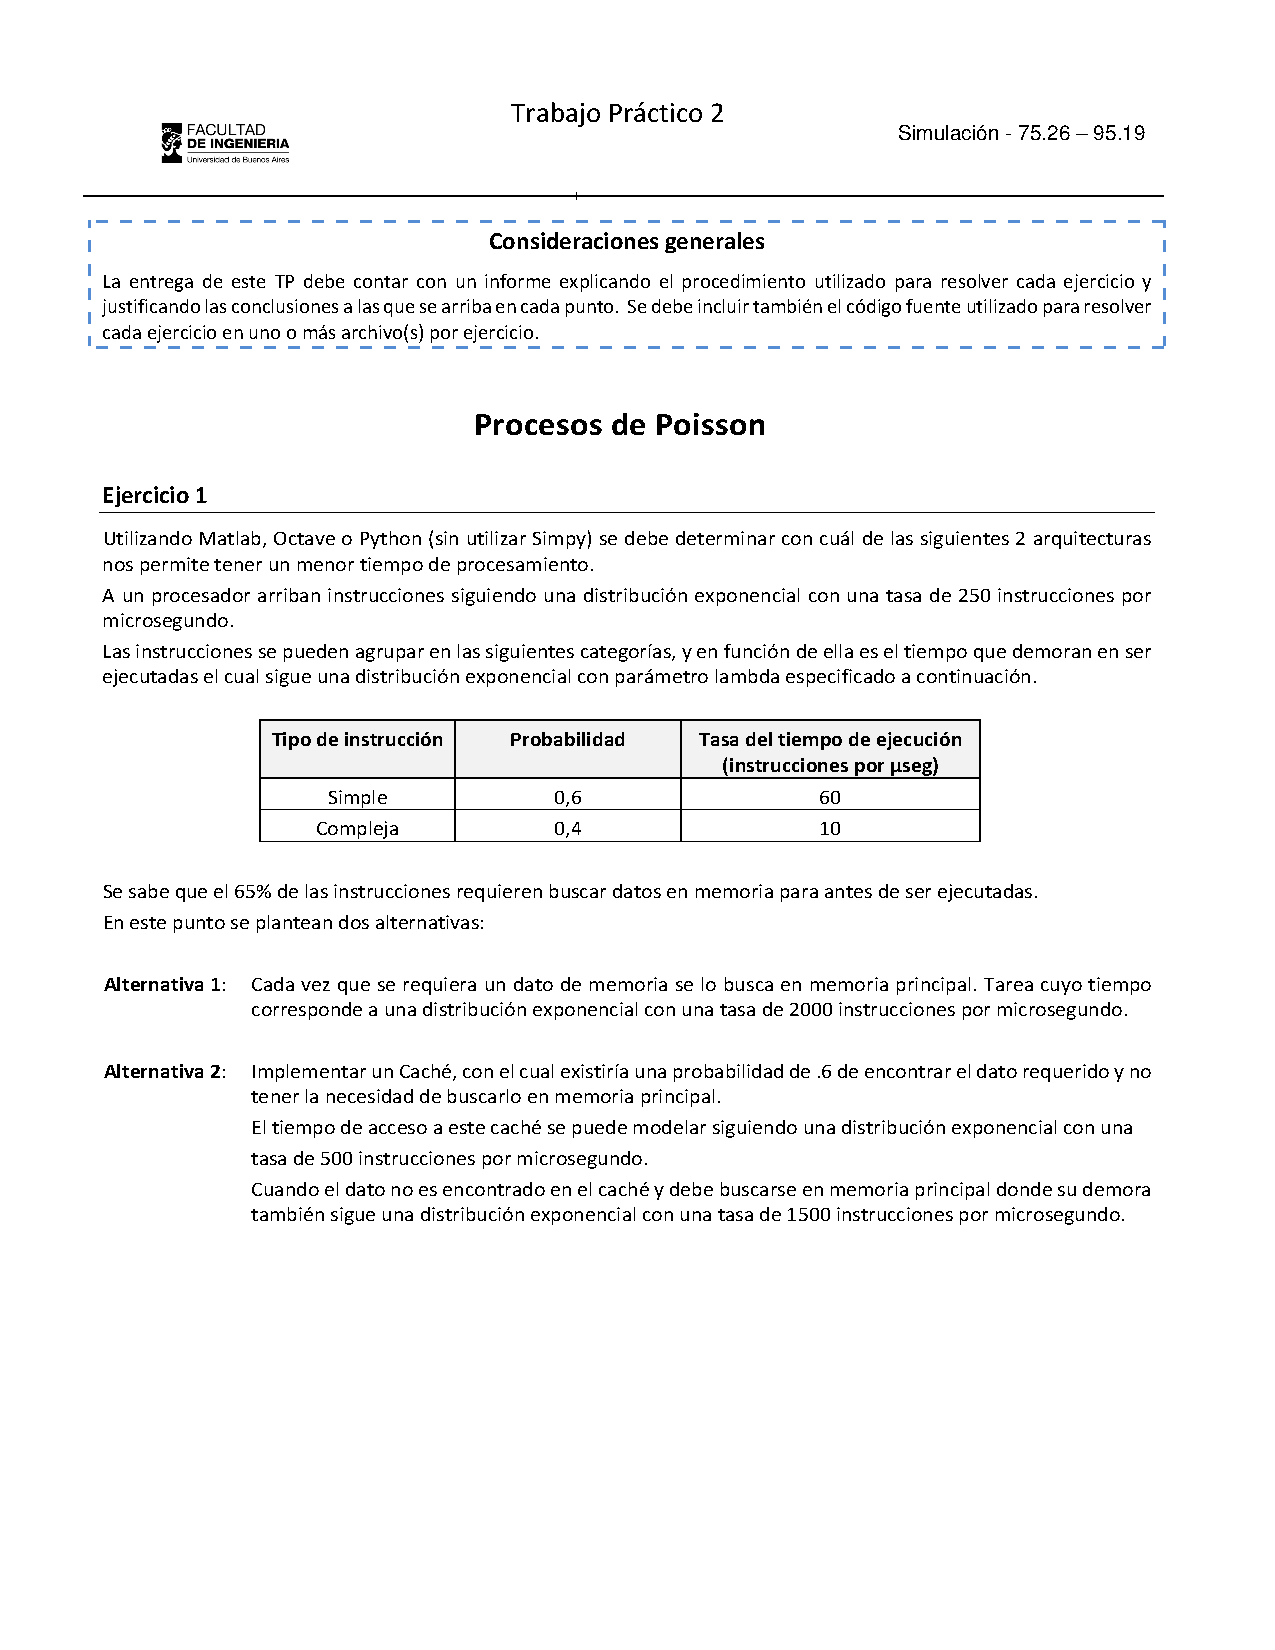
\includepdf[pages=1,scale=0.95,pagecommand = \section{Enunciado del trabajo práctico}\label{enunciado},offset=10 -10]{FIUBA-Simulacion-TrabajoPractico2.pdf}
\includepdf[pages={2},scale=0.95,pagecommand = {},offset=10 -10]{FIUBA-Simulacion-TrabajoPractico2.pdf}
\includepdf[pages={3},scale=0.95,pagecommand = {},offset=10 -10]{FIUBA-Simulacion-TrabajoPractico2.pdf}


\newpage

\section{Introducción}


\section{Implementación y resultados}
Para cada uno de los ejercicios pedidos se realiza una explicación de cada uno de ellos. Se toma como base teórica lo explicado en clase tanto teórica como clase práctica.

	\subsection{Ejercicio 1}
	    En readme.md se encuentran las instrucciones de como ejecutar el programa
	    Se utilizaron threads distintos para simular el OS que genera instrucciones, el procesador que las procesa y la memoria/cache (segun la alternativa ejecutada) que busca el dato en memoria de ser necesario, estos threads comparten una cola de instrucciones a ser ejecutadas, mientras que solo el OS y la memoria/cache comparten una cola de instrucciones que primero deben acceder a memoria

	    Los resultados obtenidos luego de ejecutar ambas alternativas durante 15 minutos fueron los siguientes:

	    \begin{figure}[H]
  			\centering
    			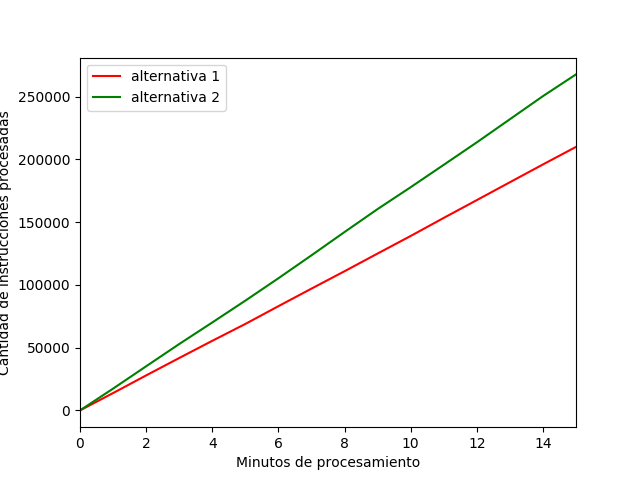
\includegraphics[width=11cm]{imagenes/ejercicio1}
		\end{figure}

		Sin duda, la mejor alternativa es la segunda. Luego de 15 minutos pudo procesar alrededor de 50mil instrucciones mas que la primer alternativa.
	\subsection{Ejercicio 2}
	    
		
	\subsection{Ejercicio 3}
		El "modelo de la telaraña" tiene la siguiente estructura:
		\begin{equation}
			\begin{array}{llllll}
				&Q_t^{demanda} = & a - bP_t \\
				&Q_t^{oferta} = & dP_{t-1} - c \\
				&Q_t^{demanda} = &Q_t^{oferta}  = &Q_t
			\end{array}
		\end{equation}
		
		En donde tienen los parámetros siguientes :
		\begin{itemize}
					\item a = 9
					\item b = 1,1
					\item c = 0,4
					\item d = 1
					\item $P_0 = 8$
		\end{itemize}

		Respondiendo lo que se pide:
		\begin{enumerate}
			\item El sistema es dicreto, lineal, autónomo y de primer orden
			\item Resolviendo el sistema de ecuaciones se obtuvo el punto de equilibrio:
				\begin{center}
					$P = \frac{a+c}{d+b}$
				\end{center}
				Utilizando los datos del ejercicio se obtuvo:
				\begin{center}
					$P = \frac{94}{21}$\\
					\vspace*{0.15in}
					$Q = \frac{428}{105}$
				\end{center}
			
			\item Realizando un análisis asintótico obtuvimos que: 
				\begin{center}
					$\lambda_1 = 1$\\
					\vspace*{0.15in}
					$\lambda_2 = \frac{-11}{10}$
				\end{center}
				En donde se llega a que el sistema es un Saddle Point.
			\item Graficando la variable precio en función del período(t):
				\begin{figure}[H]
  					\centering
    					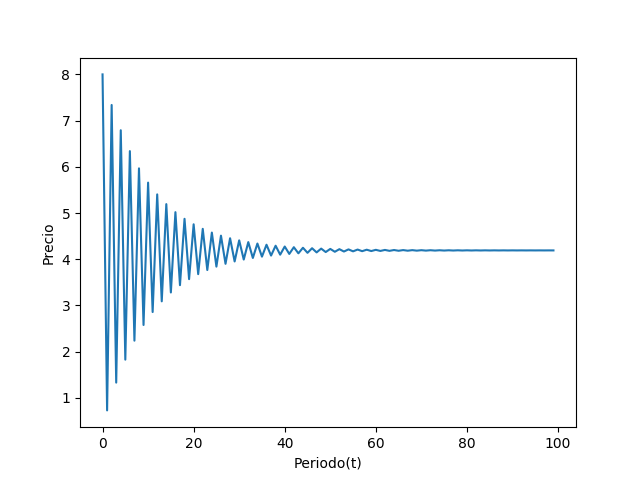
\includegraphics[width=14cm]{imagenes/precioTiempo}
				\end{figure}

		\end{enumerate}
		
		

	\subsection{Ejercicio 4}
		La conclusion es consistente con el ejercicio 1, es mejor la alternativa 2. Sin embargo por como esta implementado el ejercicio 1 nos dio distinto la cantidad de tiempo que lleva ejecutar 200000 instrucciones, para la alternativa 1 nos dio  21837124 microsegundos (alrededor de 20 segundos) y para la alternativa 2  7422610 microsegundos (alrededor de 7 segundos)
	\subsection{Ejercicio 5}
		Utilizando los datos del ejercicio procesamos nuestro archivo creado usando $Simpy$ y obtuvimos los siguientes resultados:
		\begin{itemize}
			\item Con política Round Robin(en segundos):
				\begin{itemize}
					\item Tiempo espera: 87.6
					\item Tiempo max: 416.4
					\item Tiempo min: 45.0
					\item Tiempo total: 451783.9
				\end{itemize}
			\item Las solicitudes son asignadas al azar entre los servidores:
				\begin{itemize}
					\item Tiempo espera: 73.6
					\item Tiempo max: 116.1
					\item Tiempo min: 45.0
					\item Tiempo total: 449154.5
				\end{itemize}
		\end{itemize}

		Podemos observar que la mejor política de asignación es en donde la solicitud es asignada al azar entre los 6 servidores. Hay una diferencia significativa en el tiempo máximo entre ambos y el tiempo total.

\section{Conclusiones y aclaraciones}
El trabajo práctico nos permitió conocer y realizar simulaciones teniendo como base teórica los conceptos explicados en clase . Además, nos permitió conocer herramientas que permiten realizar simulaciones que son muy utilizadas en el campo científico.

\begin{thebibliography}{10}
	\bibitem{} Python, Generación de números con distintas distribuciones de probabilidad, https://docs.python.org/3/library/random.html.
	\bibitem{} Simpy, Apunte de la cátedra.
	\bibitem{} Simpy, Documentación, https://simpy.readthedocs.io/en/latest/
	

\end{thebibliography}


\newpage
%-----------------------------------%
%									%
%			Seccion:Fuente			%
%									%
%-----------------------------------%
\appendix
\section{Código fuente}\label{appendix_codigo_fuente}

	\subsection{Resolución ejercicio 1}\label{ejercicio_1}
		\subsubsection{instruccion}
			\lstinputlisting[language=Python]{../ejercicios/Ejercicio1/instruccion.py}
		\subsubsection{cache.py}
			\lstinputlisting[language=Python]{../ejercicios/Ejercicio1/cache.py}
		\subsubsection{memoria principal}
			\lstinputlisting[language=Python]{../ejercicios/Ejercicio1/memoria_principal.py}
		\subsubsection{OS}
			\lstinputlisting[language=Python]{../ejercicios/Ejercicio1/OS.py}
		\subsubsection{procesador}
			\lstinputlisting[language=Python]{../ejercicios/Ejercicio1/procesador.py}
		\subsubsection{main}
			\lstinputlisting[language=Python]{../ejercicios/Ejercicio1/main.py}
		\subsubsection{grafico}
			\lstinputlisting[language=Python]{../ejercicios/Ejercicio1/grafico.py}

	\newpage

	\subsection{Resolución ejercicio 2}\label{ejercicio_2}
		\subsubsection{ejercicio2.py}
			%\lstinputlisting[language=Python]{../ejercicios/ejercicio2.py}

	\newpage

	\subsection{Resolución ejercicio 3}\label{ejercicio_3}
		\subsubsection{ejercicio3.py}
			\lstinputlisting[language=Python]{../ejercicios/ejercicio3.py}

	\newpage

	\subsection{Resolución ejercicio 4}\label{ejercicio_4}
		\subsubsection{ejercicio4.py}
			\lstinputlisting[language=Python]{../ejercicios/Ejercicio4/ejercicio4.py}

	\newpage

	\subsection{Resolución ejercicio 5}\label{ejercicio_5}
		\subsubsection{ejercicio5.py}
			\lstinputlisting[language=Python]{../ejercicios/ejercicio5.py}



\end{document}
